  %2017-09-13
  
  \section{Кинематика твердого тела}
  \begin{df}
  Абсолютно твердым телом называется множество точек, расстояние между которыми не меняется со временем.
  
  $  \{ \v{r_i}, i = \overline{1 \ldots n} ~~:~~|\v{r_i} - \v{r_j} | = C_{ij} = const ,~~ n \geqslant 3 \}$ 
  
  \end{df}

  \begin{figure}[h]
  \centering
  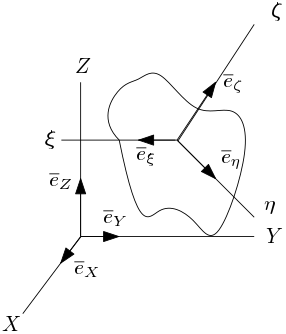
\includegraphics[width=5cm]{fig2.png} 
  \end{figure}  
  $OXYZ$ - неподвижная система отсчета.
  
  $S\xi\eta\zeta$ - связаны с телом (движется).
 
  $$
  X = 
  \left(
  \begin{matrix} 
  (\v{e_{\xi}}, \v{e_{x}}) & 
  (\v{e_{\xi}}, \v{e_{y}}) & 
  (\v{e_{\xi}}, \v{e_{z}}) \\ 
  (\v{e_{\eta}}, \v{e_{x}}) & 
  (\v{e_{\eta}}, \v{e_{y}}) & 
  (\v{e_{\eta}}, \v{e_{z}}) \\  
  (\v{e_{\zeta}}, \v{e_{x}}) & 
  (\v{e_{\zeta}}, \v{e_{y}}) & 
  (\v{e_{\xi}}, \v{e_{z}}) \\
  \end{matrix}
  \right)
  \text{ - матрица направляющих косинусов.}
  $$
 
  $$ \v{AB} = x\v{e_x} + y\v{e_y} + z\v{e_z} $$
  $$ \v{AB} = \xi\v{e_{\xi}} + \eta\v{e_{\eta}} + \zeta\v{e_{\zeta}} $$

  $$ X
  \left(
  \begin{matrix}
    x \\ y \\ z \\
  \end{matrix}
  \right)
  =
  \left(
  \begin{matrix}
  (\v{e_{\xi}}, x\v{e_x} + y \v{e_y} + z \v{e_z}) \\
  (\v{e_{\eta}}, x\v{e_x} + y \v{e_y} + z \v{e_z}) \\
  (\v{e_{\zeta}}, x\v{e_x} + y \v{e_y} + z \v{e_z}) \\
  \end{matrix}
  \right)
  = 
  \left(
  \begin{matrix}
  (\v{e_{\xi}}, \v{AB}) \\
  (\v{e_{\eta}}, \v{AB}) \\
  (\v{e_{\zeta}}, \v{AB}) \\
  \end{matrix}
  \right)
  =
  \left(
  \begin{matrix}
  \xi \\
  \eta \\
  \zeta \\
  \end{matrix}
  \right)
  =
  \v{\rho}
  $$

  $$ \v{\rho} = X \v{r} $$
  
  \begin{ass}
  $X$ - ортогональная матрица.
  \end{ass}
  \begin{proof}
  $$ XX^T = X^TX = 
  \left(
  \begin{matrix}
  (\v{e_{\xi}}, \v{e_\xi}) & 
  (\v{e_{\xi}}, \v{e_\eta}) & 
  (\v{e_{\xi}}, \v{e_\zeta}) \\
  \vdots & \ddots & \vdots \\
   & \ldots &
  \end{matrix} 
  \right)
  = E $$
  Т.к. базис ортогональный.
  \end{proof} 
  
  $$
  \left(
  \begin{matrix}
  \v{e_{\xi}} \\
  \v{e_{\eta}} \\
  \v{e_{\zeta}} \\
  \end{matrix}
  \right)  
  =  
  X
  \left(
  \begin{matrix}
  \v{e_{x}} \\
  \v{e_{y}} \\
  \v{e_{z}} \\
  \end{matrix}
  \right)
  $$

  $$
  \left(
  \begin{matrix}
  \dot{\v{e_{\xi}}} \\
  \dot{\v{e_{\eta}}} \\
  \dot{\v{e_{\zeta}}} \\  
  \end{matrix}
  \right)
  = 
  \dot{X}
  \left(
  \begin{matrix}
  \v{e_{x}} \\
  \v{e_{y}} \\
  \v{e_{z}} \\
  \end{matrix}
  \right) =
  \underbrace{
  \dot{X} X^T
  }_{\Omega}
  \left(
  \begin{matrix}
  \v{e_{\xi}} \\
  \v{e_{\eta}} \\
  \v{e_{\zeta}} \\
  \end{matrix}
  \right)
  =
  \Omega
  \left(
  \begin{matrix}
  \v{e_{\xi}} \\
  \v{e_{\eta}} \\
  \v{e_{\zeta}} \\
  \end{matrix}
  \right) 
  $$

  $$ \Omega = \dot X X^T $$

  
  \begin{ass}
  $\Omega$ - кососимметрична.
  \end{ass}
  \begin{proof}
  $$ \Omega - \Omega^T = \dot X X^T + (\dot X X^T)^T = \dot X X^T + X \dot {X^T} = \frac{d}{dt}(XX^T) = 
  \frac{d}{dt}(E) = 0 $$
  \end{proof}
  
  \begin{cor}
  $$ \Omega =
  \left(
  \begin{matrix}
  0 & \omega_{\zeta} & -\omega_{\eta} \\
  -\omega_{\zeta} & 0 & \omega_{\xi} \\
  \omega_{\eta} & -\omega_{\xi} & 0 \\
  \end{matrix}
  \right)
  $$
  \end{cor}
  --- Факт, который может быть законспектирован неправильно
  \begin{df}
  $ \v{\omega} = \omega_{\xi}\v{e_{\xi}} + \omega_{\eta}\v{e_{\eta}} + \omega_{\zeta}\v{e_{\zeta}} $ - угловая скорость подвижного репера.
  \end{df}
  
  \subsection{Формулы Пуассона}
  \begin{ass}
  $$ \dot{\v{e_i}} = [\v{\omega}, \v{e_i}],~~ i = \overline{1 \ldots 3} $$
  \end{ass}
  \begin{proof}
  $$
  \dot{\v{e_{\xi}}} = \omega_{\zeta} \v{e_{\eta}} - \omega_{\eta} \v{e_{\zeta}} =
  \begin{vmatrix}
  \v{e_{\xi}} & \v{e_{\eta}} & \v{e_{\zeta}} \\
  \omega_{\xi} & \omega_{\eta} & \omega_{\zeta} \\
  1 & 0 & 0 \\ 
  \end{vmatrix}
  =
  [\v{\omega}, \v{e_{\xi}}] 
  $$
  \end{proof}
  
  \begin{ass}
  $ \v{\omega} = \v{e_{\xi}}(\dot{\v{e_{\eta}}}, \v{e_{\zeta}}) + \v{e_{\eta}}(\dot{\v{e_{\zeta}}}, \v{e_{\xi}}) + \v{e_{\zeta}}(\dot{\v{e_{\xi}}}, \v{e_{\eta}}) $
  \end{ass}
  \begin{proof}
  $$ (\dot{\v{e_{\xi}}}, \v{e_{\eta}}) = \omega_{\zeta} $$
  $$ (\dot{\v{e_{\eta}}}, \v{e_{\zeta}}) = \omega_{\xi} $$
  $$ (\dot{\v{e_{\zeta}}}, \v{e_{\xi}}) = \omega_{\eta} $$
  \end{proof}
  
  \begin{ass}
  $ \v{\omega} = \frac{1}{2} ([\v{e_{\xi}}, \dot{\v{e_{\xi}}}] + [\v{e_{\eta}}, \dot{\v{e_{\eta}}}] + [\v{e_{\zeta}}, \dot{\v{e_{\zeta}}}]) $
  \end{ass}
  \begin{proof}
  $$ \v{\omega} 
  = \frac{1}{2} ([\v{e_{\xi}}, \dot{\v{e_{\xi}}}] + [\v{e_{\eta}}, \dot{\v{e_{\eta}}}] + [\v{e_{\zeta}}, \dot{\v{e_{\zeta}}}]) 
  = \frac{1}{2} ([\v{e_{\xi}}, [\v{\omega}, \v{e_{\xi}}]] + [\v{e_{\eta}}, [\v{\omega}, \v{e_{\eta}}]] + [\v{e_{\zeta}}, [\v{\omega}, \v{e_{\zeta}}]]) = $$
  $$ = \frac{1}{2} \left( \v{\omega}(\v{e_{\xi}}, \v{e_{\xi}}) - \v{e_{\xi}}(\v{\omega}, \v{e_{\xi}}) + \v{\omega}(\v{e_{\eta}}, \v{e_{\eta}}) - \v{e_{\eta}}(\v{\omega}, \v{e_{\eta}}) + \v{\omega}(\v{e_{\zeta}}, \v{e_{\zeta}}) - \v{e_{\zeta}}(\v{\omega}, \v{e_{\zeta}}) \right) = $$ 
  $$ = \frac{1}{2}(3\v{\omega} - \v{\omega}) = \v{\omega} $$
  \end{proof}
  
  \begin{xmp}
  Угловая скорость репера Френе.
  $$ 
  \begin{cases}
  \v{\tau}' = k \v{n} \\
  \v{n}' = - k\v{\tau} + \varkappa \v{b} \\
  \v{b}' = -\varkappa\v{n}
  \end{cases}
  $$
  
  $$
  \begin{cases}
  \dot{\v{\tau}} = \frac{d\v{\tau}}{ds} \dot s \\
  \dot{\v{n}} = \frac{d\v{n}}{ds} \dot s \\
  \dot{\v{b}} = \frac{d\v{b}}{ds} \dot s \\
  \end{cases} 
  $$
  
  $$ \v{\omega} = \v{\tau}(\dot s (-k\v{\tau} + \varkappa\v{b}), \v{b}) + \v{n}(\dot s (-\varkappa\v{n}, \v{\tau}) + \v{b}(\dot s(k \v{n}), \v{n}) = \dot s (\varkappa\v{\tau} + k\v{b}) $$
  \end{xmp}
  
  \begin{df}
  Угловой скоростью твердого тела называется угловая скорость подвижного репера, с ним связанного.
  \end{df}
 
  \subsection{Формула распределения скоростей точек твердого тела (Формула Эйлера)}
  \begin{figure}[H]
  \centering
  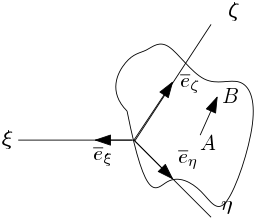
\includegraphics[width=5cm]{fig3.png} 
  \end{figure}  
  $$ \v{v_B} = \v{v_A} + [\v{\omega}, \v{AB}] $$
  
  \begin{proof}
  $$ \v{AB} = \xi \v{e_{\xi}} + \eta \v{e_{\eta}} + \zeta \v{e_{\zeta}} $$
  $$ \dot{\v{AB}} = \xi \dot{\v{e_{\xi}}} + \eta \dot{\v{e_{\eta}}} + \zeta \dot{\v{e_{\zeta}}},~~ \dot{\xi} = \dot{\eta} = \dot{\zeta} = 0 $$
  $$ \dot{\left(\v{r_B} - \v{r_A}\right)}~~ = \xi[\v{\omega}, \v{e_{\xi}}] + \eta[\v{\omega}, \v{e_{\eta}}] + \zeta[\v{\omega}, \v{e_{\zeta}}] $$ 
  $$ \dot{\v{r_B}} - \dot{\v{r_A}} = [\v{\omega}, \xi \v{e_{\xi}} + \eta \v{e_{\eta}} + \zeta \v{e_{\zeta}}] $$
  $$ \v{v_B} = \v{v_A} + [\v{\omega}, \v{AB}] $$  
  \end{proof}
  
  \begin{cor}
  $S\xi\eta\zeta \rightarrow \v{\omega}$, $S'\xi'\eta'\zeta' \rightarrow \v{\omega}'$
  $$ 
  \left.
  \begin{array}{ccc}
  \v{v_B} = \v{v_A} + [\v{\omega}, \v{AB}] \\
  \v{v_B} = \v{v_A} + [\v{\omega'}, \v{AB}]
  \end{array}
  \right|
  [\v{\omega} - \v{\omega}', \v{AB}] = 0;~ \forall A, B \text{ в абсолютно твердом теле} \Rightarrow
  $$
  $$ \Rightarrow \v{\omega} - \v{\omega}' = 0 \Rightarrow \boxed{\v{\omega} = \v{\omega}'} $$
  \end{cor}
  
  \begin{ass}(Формула Ривальса) $ \v{w_B} = \v{w_A} + [\v{\varepsilon}, \v{AB}] + [\v{\omega}, [\omega, \v{AB}]] $.
  \end{ass}
  \begin{proof}
  $$ \v{v_B} = \v{v_A} + [\v{\omega}, \v{AB}] $$
  $$ \dot{\v{v_B}} = \dot{\v{v_A}} + [\dot{\v{\omega}}, \v{AB}] + [\v{\omega}, \dot{\v{r_B} - \v{r_A}}~]  $$
  $$ \v{w_B} = \v{w_A} + [\v{\varepsilon}, \v{AB}] + [\v{\omega}, [\v{\omega}, \v{AB}]]  $$
  $$ [\v{\varepsilon}, \v{AB}] \text{ - вращательное ускорение,~~} [\v{\omega}, [\v{\omega}, \v{AB}]] \text{ - осестремительное ускорение} $$ 
  \end{proof}
  
  \subsubsection*{Геометрический смысл $\v w_{OC}$}
  \begin{figure}[H]
  \centering
  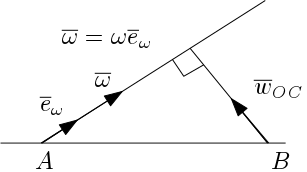
\includegraphics[width=5cm]{fig4.png} 
  \end{figure}
  $ \v{w} = [\v{\omega}, [\v{\omega}, \v{AB}]] = \v{\omega} (\v{\omega}, \v{AB}) - \v{AB} \omega^2 = \omega^2 ( \v{e_{\omega}}(\v{AB}, \v{e_{\omega}}) - \v{AB}) $
  
  $ | \v{w_{\textbf{ос}}} |= \omega^2 \rho(B, l) $
  
  \begin{ass}
  Проекции скоростей двух точек твердого тела на прямую, их соединяющую, равны.
  \begin{figure}[H]
  \centering
  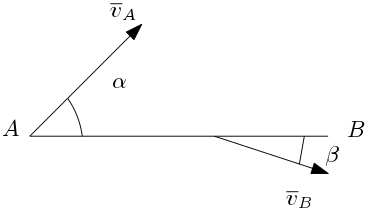
\includegraphics[width=5cm]{fig5.png} 
  \end{figure}
  \end{ass}
  \begin{proof}
  $$ \v{v_B} = \v{v_A} + [\v{\omega}, \v{AB}] $$
  $$ (\v{v_B}, \v{AB}) = (\v{v_A}, \v{AB}) + ([\v{\omega}, \v{AB}], \v{AB}) $$
  $$ v_B \cos \beta = v_A \cos \alpha $$
  \end{proof}
  \begin{ntc}
  Аналогичная теорема для ускорений не верна.
  \end{ntc}
  
  \section{Классификация движения твердого тела}
  
  \subsection{Поступательное движение}
  \begin{df}
  Такое движение твердого тела, при котором угловая скорость равна нулю.
  \end{df}
  \begin{figure}[H]
  \centering
  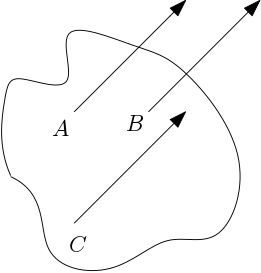
\includegraphics[width=5cm]{img/fig6.png} 
  \end{figure}
  $$ \v{v_B} \equiv \v{v_A} $$
  $$ \v{w_B} \equiv \v{w_A} $$
  \paragraph{Мгновенное поступательное движение:}
  $ \exists t : \v{\omega}(t) = 0,~~ \v{\varepsilon}(t) \neq 0 $
  
  \subsection{Вращательное движение (вращение вокруг неподвижной оси)}
  ~
  $$ \exists A, B : \v{v_A} = \v{v_B} = 0 $$
  \begin{figure}[H]
  \centering
  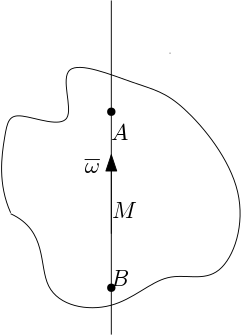
\includegraphics[width=5cm]{img/fig7.png} 
  \end{figure}
  \begin{flalign*}
  & \v{v_B} = \v{v_A} + [\v{\omega}, \v{AB}], \v{v_A} = \v{v_B} = 0 \Rightarrow [\omega, \v{AB}] = 0 \Rightarrow \omega \parallel \v{AB} &\\
  & \forall M \in l : \v{v_M} = 0 \text{, $l$ - ось вращения} &\\
  & \dot{\vec{e}}_{\xi} = \dot{\varphi} \vec{e}_{\eta},~ \dot{\vec{e}}_{\eta} = -\dot{\varphi} \vec{e}_{\xi},~ \dot{\vec{e}}_{\zeta} = 0  &\\
  & \vec{\omega} = \vec{e}_{\xi}(-\dot{\varphi}\vec{e}_{\xi}, \vec{e}_{\zeta}) + \vec{e}_{\eta}(0, \vec{e}_{\xi}) + \vec{e}_{\zeta}(\dot{\varphi} \vec{e}_{\eta}, \vec{e}_{\eta}) = \dot{\varphi} \vec{e}_{\zeta} = \dot{\varphi}\vec{e}_{z} &\\
  & \vec{\varepsilon} = \dot{\vec{\omega}} = \ddot{\varphi}\vec{e}_z &\\
  & \vec{v}_p = \vec{v}_{p'} + [\vec{\omega}, \overline{pp'}] = 0 + [\dot{\varphi}\vec{e}_z, \xi\vec{e}_{\xi} + \eta\vec{e}_{\eta}] = \dot{\varphi}(\xi\vec{e}_{\eta} - \eta\vec{e}_{\xi}) &\\
  & | \vec{v}_p | = | \vec{\omega} | \cdot | \overline{p'p} | &\\
  & \vec{w}_p = \vec{w}_{p'} + [\vec{\varepsilon}, \overline{p'p}] + [\vec{\omega}, [\vec{\omega}, \overline{p'p}]] = 0 + [\vec{\varepsilon}, \overline{p'p}] - \omega^2 \overline{p'p} &\\
  \end{flalign*}
 